\documentclass[12pt, a4paper]{article}

\usepackage[utf8]{inputenc}
\usepackage{graphicx}
\usepackage{multirow}
\usepackage{multicol}
\usepackage{subcaption}
\usepackage{mathtools}
\usepackage{amsmath}
\usepackage{authblk}
\usepackage[left=0.8in,right=0.8in,top=1in,bottom=1in ]{geometry}
\title{CSE 300: Online Assignment}

\author[1, *]{Shehabul Islam Sawraz}
\author[1, $\dagger$]{Abrar Nafee Akhand}
\author[1, $\dagger$]{Mobaswirul Islam}
\author[1, $\dagger$]{Fardin Anam Aungon}
\affil[1]{Department of Computer Science and Engineering \newline
	Bangladesh University of Engineering and Technology}
\affil[*]{Corresponding author: shehabulislamsawraz@gmail.com}
\affil[$\dagger$]{These authors contributed equally to this work}


\date{July 21, 2022}
\begin{document}
	
	\maketitle
	
	\section{Introduction}
	This assignment has been designed to assess the preparation of the students in writing
	scientific articles using \LaTeX. This assignment covers a variety of components that are
	commonly used in scientific manuscripts.
	
	\subsection{Tables}
	We wish to place Table \ref{table:1} right here.
	\begin{table}[h]
		
		\centering
		\caption{\textbf{Optimization scores for Method-1 and Method-2 on different datasets
				covering various model conditions.} We show average scores of two optimization
			criteria for various model conditions.}
		\label{table:1}
		\begin{tabular}{|c| c c | c c | c c|}
			\hline
			
			\multicolumn{3}{|c|}{Simulation Condition} & \multicolumn{4}{|c|}{Optimization Score} \\
			\hline
			\multirow{2}{*}{Dataset} & \multirow{2}{*}{Complexity} & \multirow{2}{*}{Model Condition} & \multicolumn{2}{|c|}{Score 1} & \multicolumn{2}{|c|}{Score 2} \\
			\cline{4-7} 
			& & & Method-1 & Method-2 & Method-1 & Method-2 \\ 
			\hline
			\hline
			\multirow{4}{*}{D1} & \multirow{2}{*}{Easy} & M1 & 7,425.55 & 770.00 & 929.55 & 10 \\
			&  & M2 & 7,657.00 & 9,179.00 & 716.15 & 20 \\
			\cline{2-7}
			& \multirow{2}{*}{Hard} & M3 & 54.00 & 9,007.15 & 3,759.00 & 30 \\
			&  & M4 & 74.00 & 5567.15 & 99.00 & 25 \\
			\hline
			\hline
			\multirow{3}{*}{D2} & \multirow{3}{*}{Moderate} & M1 & 34.00 & 273.00 & 321.60 & 34 \\
			&  & M2  & \multicolumn{2}{|c|}{Not Applicable} & 16.00 & 11 \\
			& & M3 & 657.00 & 179.60 & 716.00 & 19 \\
			\hline
			
		\end{tabular}
	\end{table}
	\pagebreak
	\subsection{Figures}
	We intend to put Figure \ref{fig:1} at the top of a page.
	\subsection{Equations}
	Let $n_1 |n_2 |n_3$ be a tripartition defined on an internal node $u$ of a binary tree $T$. The
	number of tripartitions mapped to $u$ is given by Eqn. \ref{eqn: 1}.
	\begin{equation}
		\label{eqn: 1}
		\begin{aligned}
			\mathcal{N} \mathcal{Q}(n_1, n_2, n_3) 
			& ={{n_1}\choose{2}} {{n_2}\choose{1}} {{n_3}\choose{1}} + {{n_2}\choose{2}} {{n_1}\choose{1}} {{n_3}\choose{1}} + {{n_3}\choose{2}} {{n_1}\choose{1}} {{n_2}\choose{1}} \\
			& = \frac{n_1n_2n_3(n_1+n_2+n_3-3)}{2}
		\end{aligned}	
	\end{equation}
	
	\subsection{Equations2}
    Let C be a simple piecewise smooth curve that bounds a region D in the plane. If $P(x, y)$ and $Q(x, y)$ have continuous partials in an open region containing D, then\linebreak
    $\int_C P \,dx + Q \,dy = \iint_D \frac{\partial Q}{\partial x} - \frac{\partial P}{\partial y}$
    \par
    If \textbf{F} is a vector field with third component 0 defined on a domain D enclosed by boundary C then\linebreak
    $ \oint\limits_C \VF{F}\cdot \,dr = \iint\limits_D (\nabla \times \VF{F})\cdot k \dif A $
    \par
    Similarly, if C is defined by $\VF{r}(t) = \langle x(t), y(t) \rangle$\linebreak
    $ \oint\limits_C \VF{F}\cdot \,dx  = \iint\limits_D \nabla \cdot \VF{F}\dif A $
    
    
	\begin{figure}[t]
		\centering
		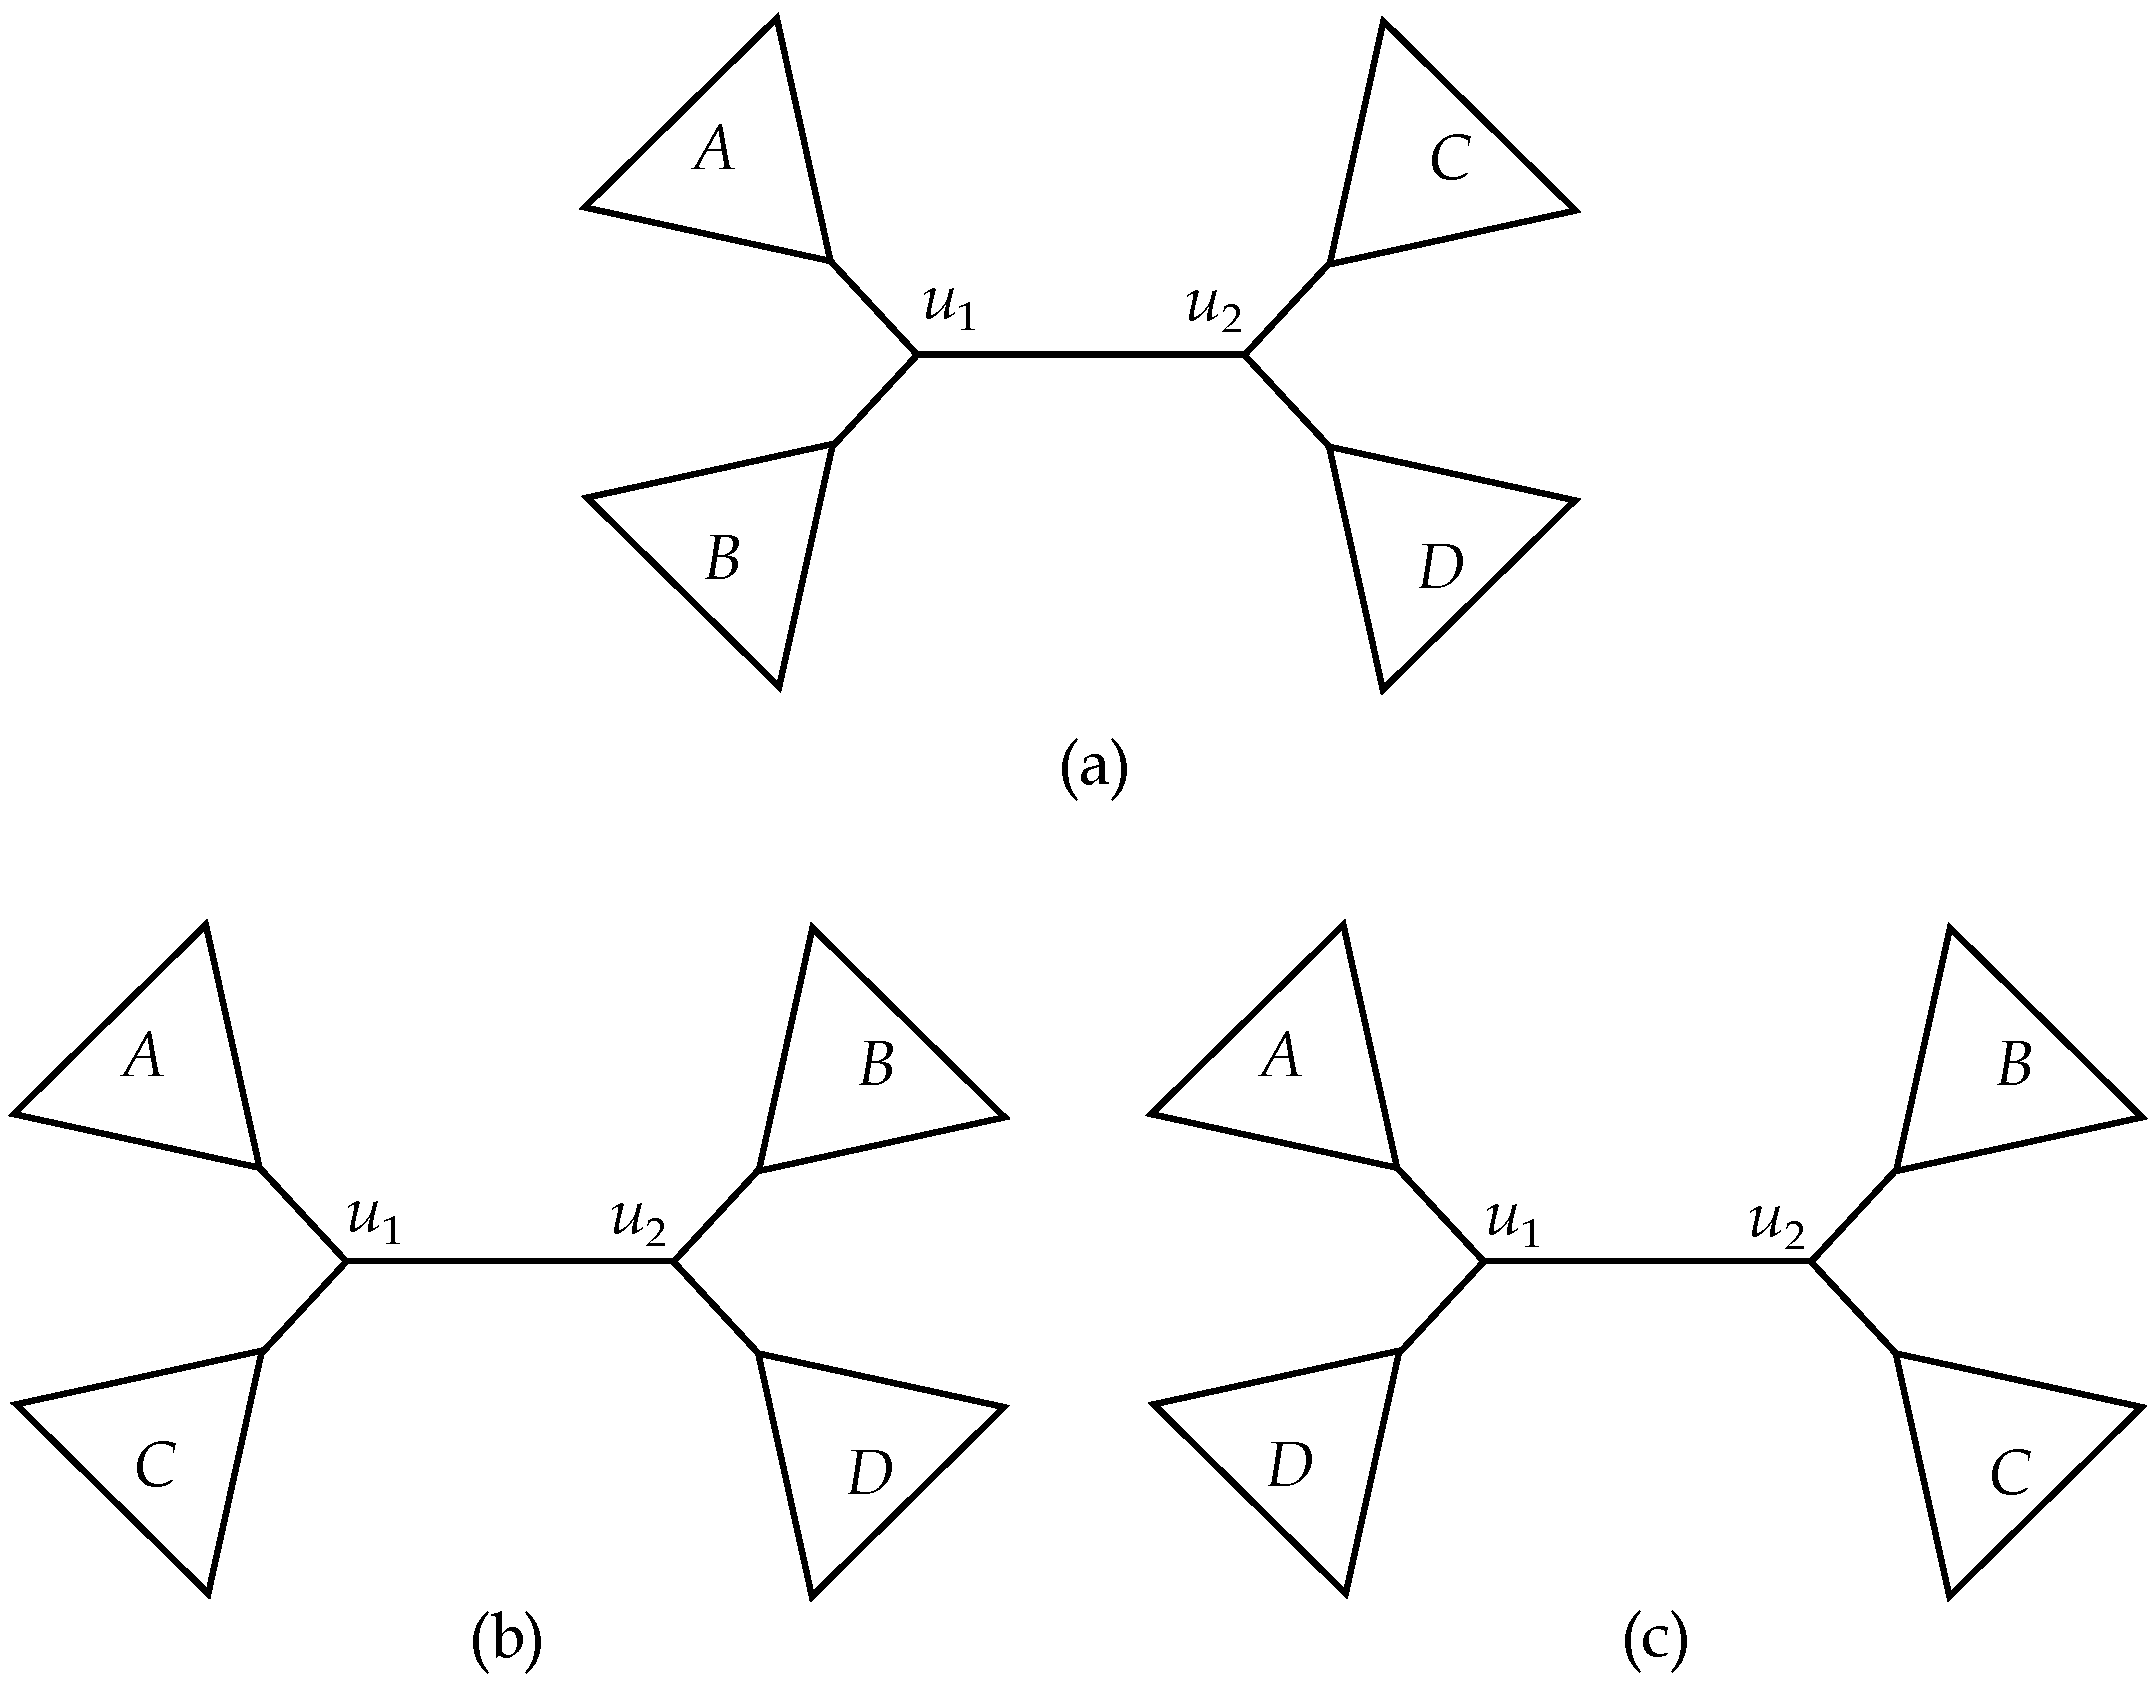
\includegraphics[scale=0.35]{Figure3.pdf}
		\caption{\textbf{Nearest Neighbor Interchange (NNI) move on an internal edge.}
			(a)A species tree ST , and 
			(b-c)the neighbors of ST resulting from one NNI move on edge
			$e = (u_1 , u_2 )$. \textit{A, B, C,} and \textit{D} are the sets of taxa in the four subtrees around edge \textit{e}.}
		
		\label{fig:1}
	\end{figure}
	\section{Conclusions}
	The major objectives of this assignment are listed below (please do not ignore the font
	sizes).
	\begin{itemize}
		\item\Huge{To see if the students have adequately practiced different aspects of
			writing in \LaTeX.}
		\item\Large{To assess the ability of the students in preparing manuscripts
			in \LaTeX.}
		\item\normalsize {To see if the students can add various basic components (e.g., tables, figures, equations) to a {\LaTeX}  manuscript.}
		\item To see if the students can leverage the available materials (both offline and online) to do
		something which has not explicitly been taught in the class.
	\end{itemize}
	
	\begin{table}[b]
    \centering
    \begin{tabular}{|l||l|l|l|}
    \hline
    \multicolumn{4}{|c|}{Item List} \\ \hline
    Item Name or & \multirow{2}{*}{ALPHA 2 Code} & \multirow{2}{*}{ALPHA 3 Code} & \multirow{2}{*}{Numeric Code} \\ \cline{1-1}
    Product Name &  &  &  \\ \hline
    \multirow{2}{*}{Item001} & \multirow{2}{*}{AF} & \multirow{2}{*}{AFG} & 001 \\
    &  &  & 002 \\ \hline
    Item002 & AX & ALA & 003 \\ \hline
    \multirow{4}{*}{Item003} & \multirow{4}{*}{AL} & \multirow{4}{*}{ALB} & 004 \\
    &  &  & 005 \\
    &  &  & 006 \\
    &  &  & 008 \\ \hline
    \multirow{2}{*}{Item004} & \multirow{2}{*}{DZ} & \multirow{2}{*}{DZA} & 009 \\
    &  &  & 010 \\ \hline
    \multirow{2}{*}{Item005} & \multirow{2}{*}{AS} & \multirow{2}{*}{ASM} & 011 \\
    &  &  & 012 \\ \hline
    Item006 & AD & AND & 013 \\ \hline
    Item007 & AO & AGO & 014 \\ \hline \hline
    \end{tabular}
    \end{table}
    \pagebreak
    \begin{figure}[t]
            \centering
            \begin{subfigure}[b]{0.7\linewidth}
                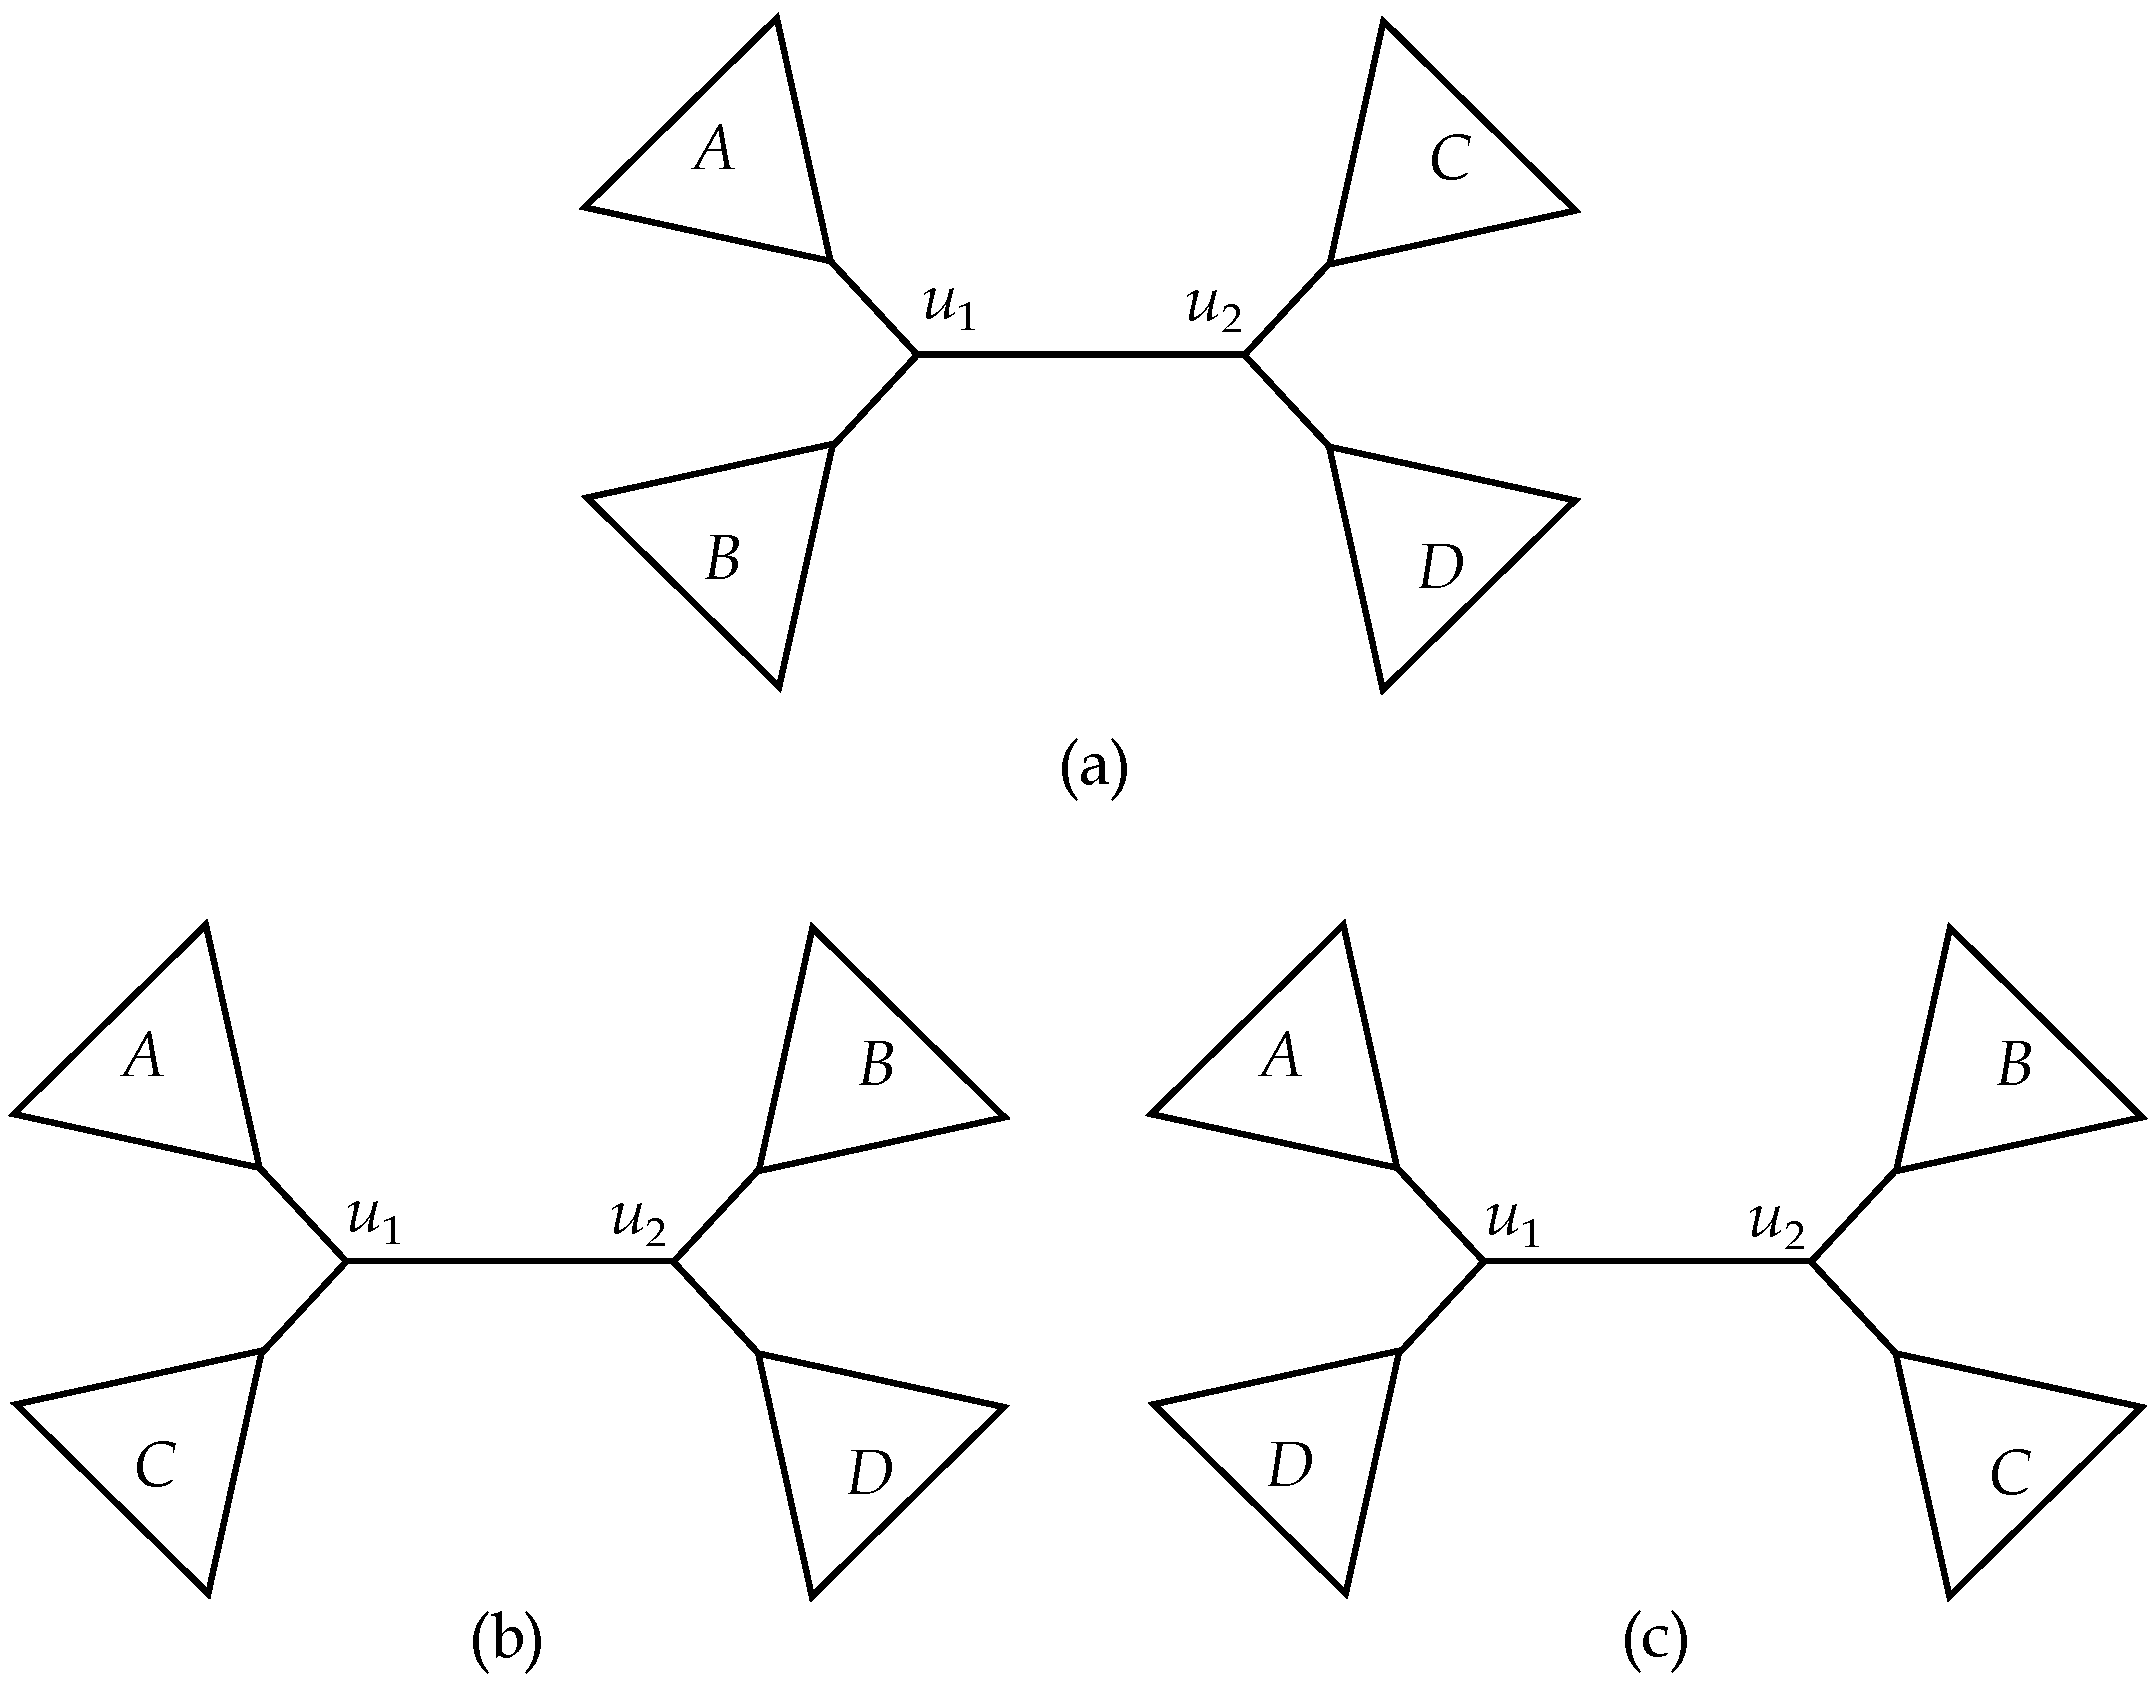
\includegraphics[width=\linewidth, angle=180]{Figure3.pdf}
            \end{subfigure}
            \begin{subfigure}[b]{0.7\linewidth}
                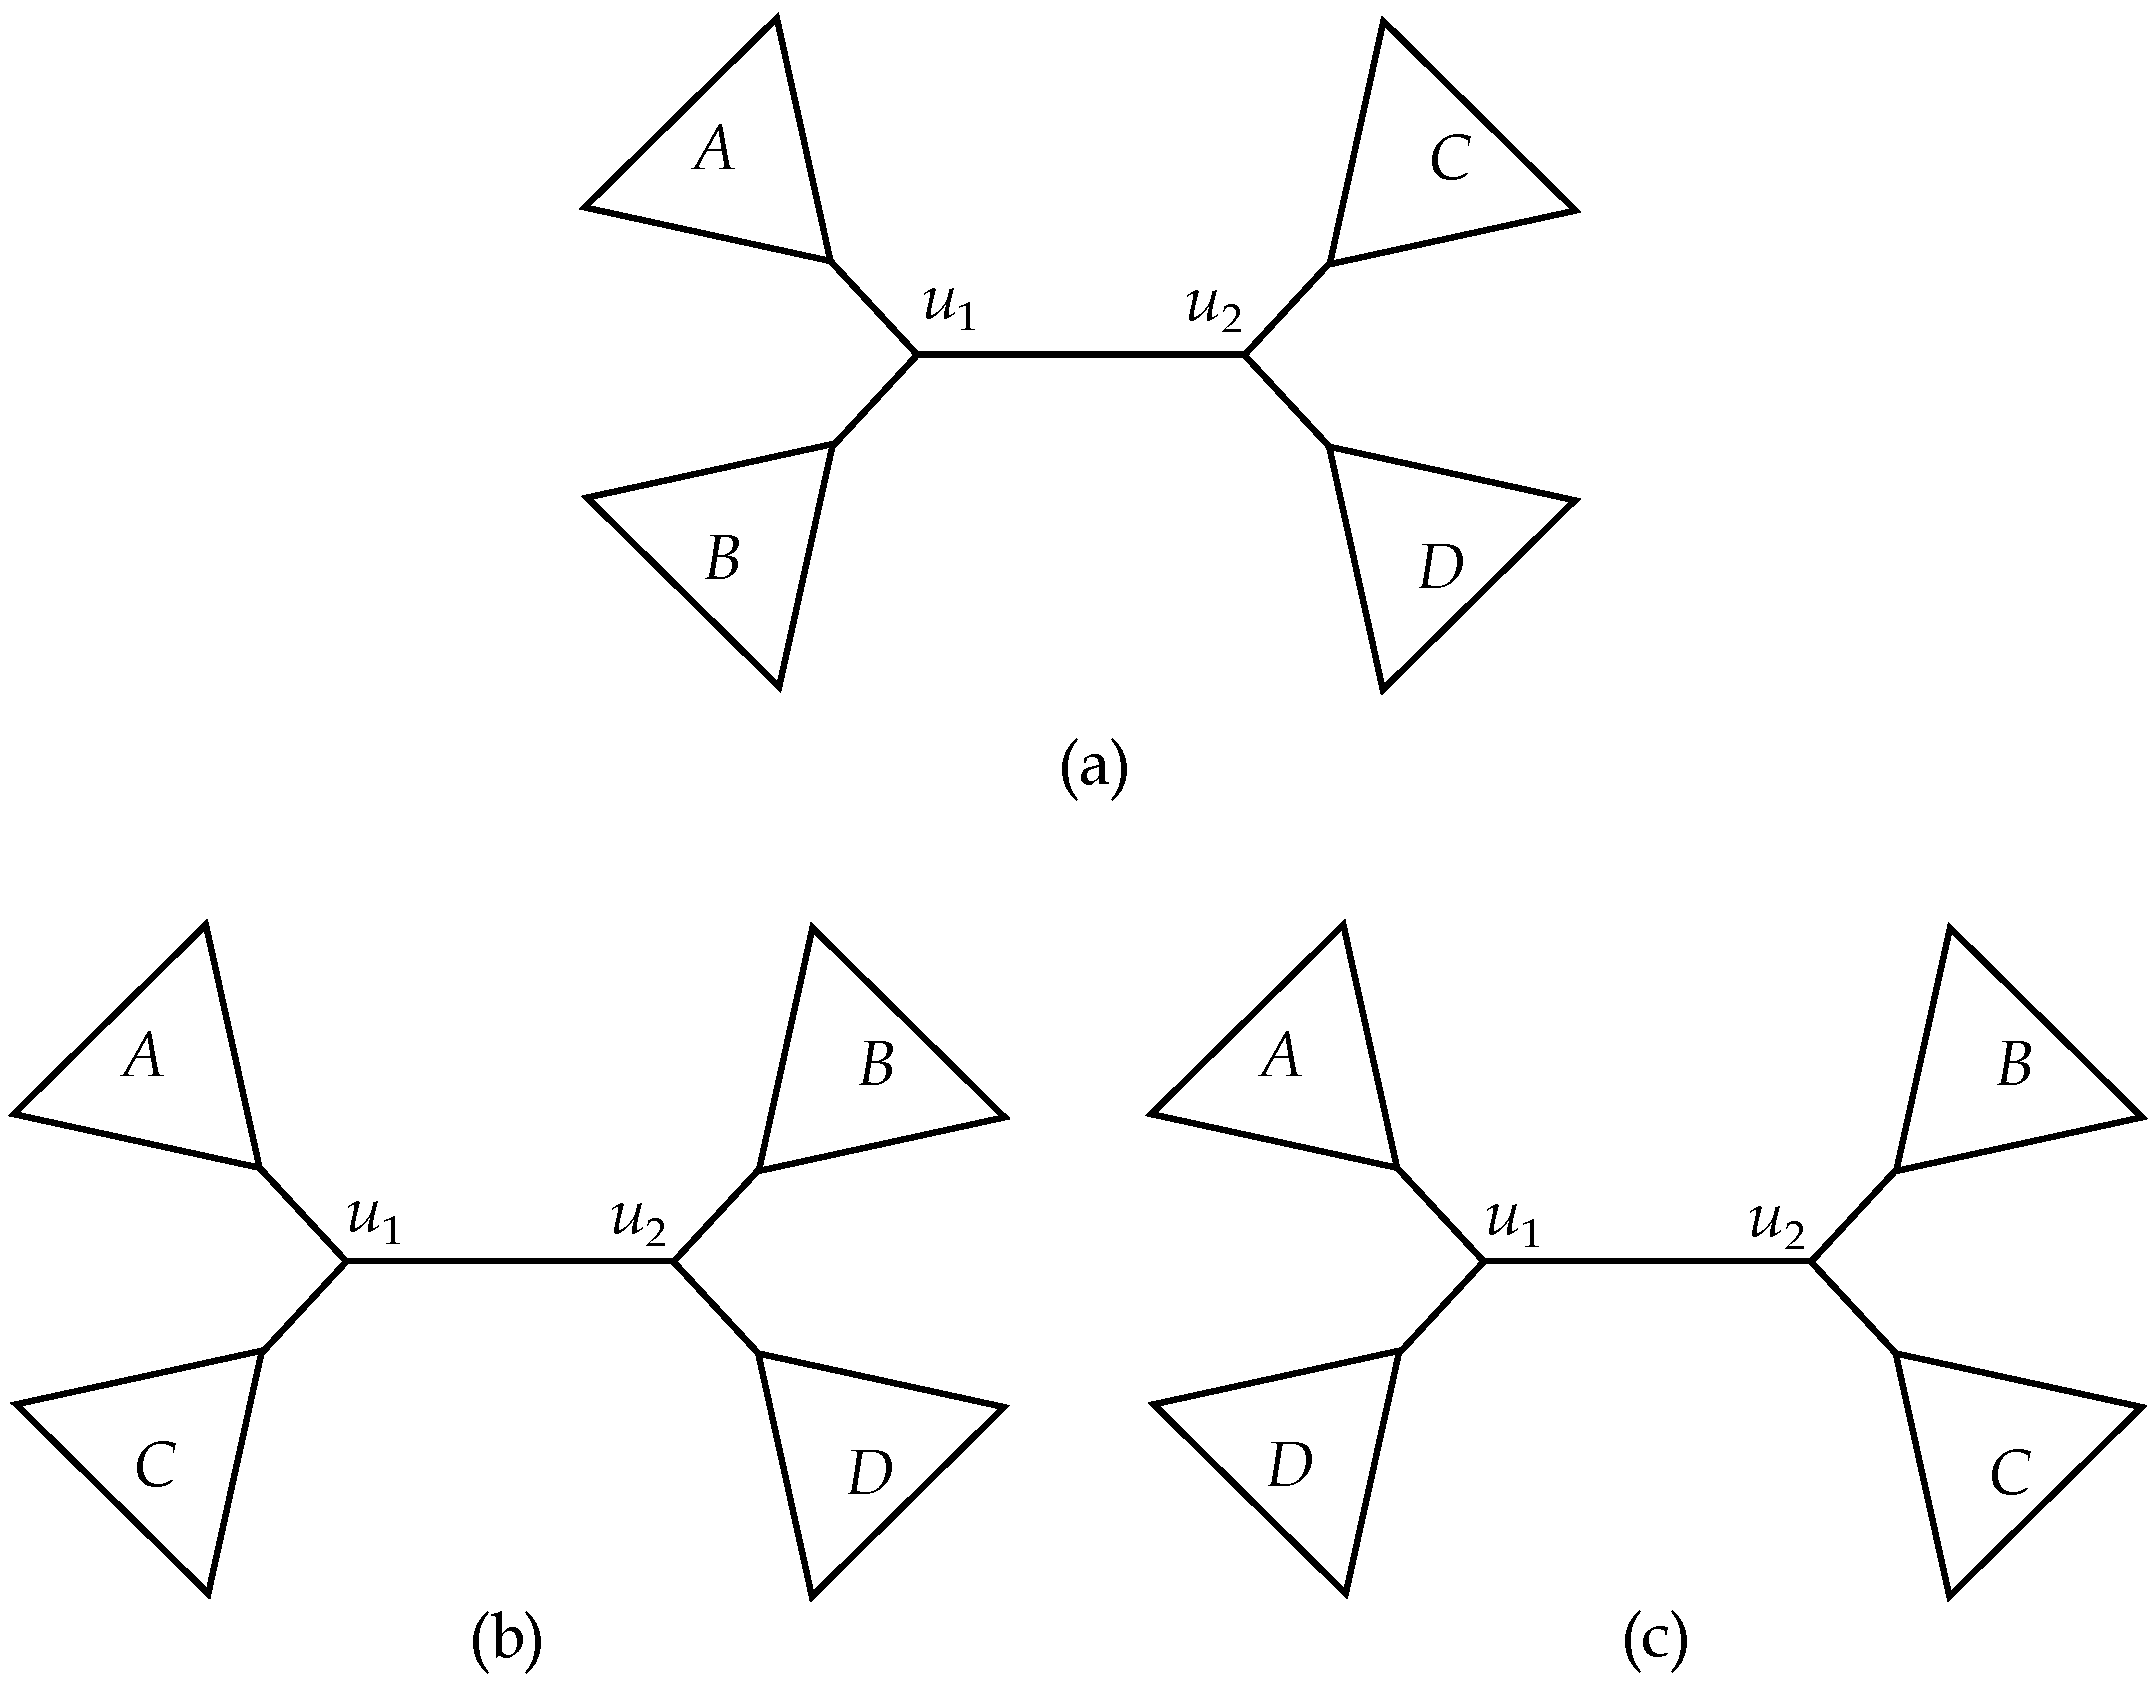
\includegraphics[width=\linewidth]{Figure3.pdf}
            \end{subfigure}
            \caption{\label{fig:fig1}\textbf{Same figure upside down}}
    \end{figure}
\end{document}
